% Chapter Template

\chapter{Scenario} % Main chapter title

\label{Chapter3} % Change X to a consecutive number; for referencing this chapter elsewhere, use \ref{ChapterX}

\textit{In questo capitolo facciamo un introduzione su quello che è lo scenario che stiamo considerando per il nostro lavoro: 
quello delle comunicazioni satellitare. Vediamo nel dettaglio quali sfide introduce, le tecnologie utilizzate 
e come affrontare le possibile problematiche a causa di applicare la PQC.}

%----------------------------------------------------------------------------------------
%	SECTION 1
%----------------------------------------------------------------------------------------

\section{Comunicazioni Satelliari}


Le comunicazioni satellitari sono fondamentali per le infrastrutture moderne, poichè abilitano una vasta gamma di servizi.
Negli ultimi decenni, con l'aumento della domanda di connettività globale e l'espansione delle reti di comunicazione, i satelliti sono diventati strumenti essenziali per garantire una copertura estesa.
L'emergere delle costellazioni di satelliti in orbita bassa (LEO - Low Earth Orbit) sta cambiando il paradigma delle comunicazioni satellitari, offrendo vantaggi significativi rispetto ai satelliti geostazionari (GEO), un confronto tra le due orbite è mostrato in \textit{Figura \ref{fig:orbite}}. 
%Mentre i satelliti GEO forniscono una copertura stabile, i satelliti LEO consentono Round Time Trip (RTT) notevolmente ridotti e una maggiore flessibilità, rendendoli ideali per applicazioni ad alta velocità come la trasmissione dati in tempo reale e la connettività Internet globale.
\todo{Scrivere meglio questa parte finale}
Questo cambio di paradigma insieme al quantum computer hanno portato diversi enti, tra cui l'Agenzia Spaziale Europea (ESA), ad affrontare nuove sfide.

\begin{figure}[h!]
    \centering
    \begin{tikzpicture}
        % Definizione dei colori per le orbite
        \definecolor{leo}{gray}{0.2}    % Grigio scuro
        \definecolor{geo}{gray}{0.1}% Grigio molto scuro
        \definecolor{terra}{HTML}{008F39}
        \node at (-4.8, 0) [color=geo]{GEO};
        \node at (3.5, 0) [color=leo]{LEO};
        \node at (0, 0) {Terra};
        
        \draw[thick, dashed, geo] (0,0) circle (4.2cm);
        \draw[thick, dashed, leo] (0,0) circle (3cm);
        \filldraw[fill=mare,] (0,0) circle (2.2cm);

        \path[draw, decoration={text along path, text={$2.000km$}, text align=center}, decorate] (0,0) (180:2.8cm) arc (180:360:2.8cm);
        \path[draw, decoration={text along path, text={$36.000km$}, text align=center}, decorate] (0,0) (180:4cm) arc (180:360:4cm);

        \node at (-2.5,2) {\includegraphics[width=1cm]{Figures/satellite.png}}; % Sostituisci 'your_image.png' con il percorso della tua immagine
        \node at (3.2,3) {\includegraphics[width=1cm, angle=270]{Figures/satellite.png}}; % Sostituisci 'your_image.png' con il percorso della tua immagine
        \node at (0.2,0.5) {\includegraphics[width=3cm ]{Figures/europe.png}}; % Sostituisci 'your_image.png' con il percorso della tua immagine

        \node[cloud, cloud puffs=15.7, cloud ignores aspect, minimum width=1.5cm, minimum height=0.5cm, align=center, fill=white, draw] (cloud) at (-2, 0) {};
        \node[cloud, cloud puffs=15.7, cloud ignores aspect, minimum width=1.5cm, minimum height=0.5cm, align=center, fill=white, draw] (cloud) at (2, -0.5) {};

    \end{tikzpicture}
    \caption{Orbite dei satelliti}
    \label{fig:orbite}
\end{figure}

\subsection{Limitazioni}

L'ambiente spaziale, caratterizzato da radiazioni intense, temperature estreme e lunghi periodi senza manutenzione, pone sfide significative in termini di progettazione e operatività dell'hardware e del software.
Tra i principali vincoli per l'hardware satellitare troviamo:

\begin{itemize}
    \item \textit{Resistenza alle radiazioni}: i componenti elettronici sono progettati per resistere all'esposizione costante alle radiazioni spaziali.
    \item \textit{Basso consumo energetico}: l'energia disponibile per le operazioni risulta limitata, quindi si usano processori a basso consumo e ad alta efficienza energetica, sacrificando potenza di calcolo.
    \item \textit{Elaborazione in tempo reale}: per alcune tipologie di servizi è necessario che il processamento avvenga in tempo reale.
    \item \textit{Compattezza}: a causa dello spazio limitato a bordo di un satellite, i componenti hardware devono essere progettati in modo estremamente compatto.
\end{itemize}

\noindent
L'hardware limitato ha un impatto diretto sullo sviluppo del software per i satelliti. 
Rispetto al un contesto terrestre, dove le risorse computazionali sono abbondanti, il software per i satelliti deve essere ottimizzato per funzionare su processori con bassa potenza di calcolo e memoria ridotta. 
Le principali sfide per gli sviluppatori sono:

\begin{itemize}
    \item \textit{Semplicità e ottimizzazione}: gli algoritmi devono essere semplici e ottimiz\-zati per funzionare su hardware con risorse limitate.
    \item \textit{Parallelismo limitato}: le operazioni devono essere eseguite in modo lineare o con limitato parallelismo, aumentando la complessità della progettazione.
    \item \textit{Affidabilità assoluta}: il software deve essere robusto, sicuro e testato ampiamente in modo tale che possibile errori non abbiano conseguenza catastrofiche.
\end{itemize}

\noindent
È fondamentale prestare particolare attenzione alle implementazioni 
crittogra\-fiche dato che in contesto come questo, risulta cruciale trovare un equilibrio tra
sicurezza e prestazioni. Da un lato, è necessario proteggere le comunicazioni
utilizzando algoritmi crittografici complessi; dall'altro, è essenziale
garantire che le operazioni eseguite non compromettano l'operatività del
satellite.

\subsection{Stato Attuale}

Per capire quale è la differenza in termini di hardware e software rispetto a quelli a cui siamo abiutati 
introduciamo quelli che sono gli attuali standard impiegati in questo settore.

\begin{itemize}
    \item Tra i processori utilizzati abbiamo \textit{LEON3}, un processore open-source basato sull'architettura SPARC, progettato dall'ESA. 
    \item ESA Power Interface Standard (ECSS-E-ST-20C): definisce come deve avvenire la distribuituzione dell'alimentazione elettrica all'interno dei satelliti.
    \item Cubesat Standard: definisce dimensioni compatte modulari (10x10x10 cm per 1U) per ridurre i costi e semplificare il lancio e la costruzione dei satelliti.
    \item Triple Modular Redundancy (TMR): nei sistemi critici spaziali si utilizza la ridondanza tripla modulare, per garantire l'affidabilità dei risultati tramite sistemi di voting.
\end{itemize}
\noindent
Il sistema operativo utilizzato in queste applicazioni è RTEMS (Real-Time Executive for Multiprocessor Systems) che le caratteristiche di essere open-source, real-time e basato su GNU/Linux.
\todo{se si trova riportare qualche riferimento}

%-----------------------------------
%	SECTION 2
%-----------------------------------
\subsection{Sfide}
\noindent
Per rendere le comunicazioni satellitari sicure ad attacchi Qauntum occorre adottare algoritmi più complessi.
Questi utilimi, tuttavia, oltre a richiedere più memoria per la gestione delle chiavi,
comportano un incremento significativo del carico di calcolo. Le sfide da affrontare sono:

\begin{itemize}
    \item  Aumento complessità computazionale: l'incremento delle dimensioni delle chiavi e della complessità degli algoritmi portano a un aumento del carico computazionale. Aggiungendo ulteriori vincoli su sistemi già limitati. 
    \item Incremento della larghezza di banda necessaria: oltre all'aumento di carico si ha anche magiore utilizzo della larghezza di banda, che in comunicazioni satellitari risuta già limitata.
    \item Compatibilità retroattiva: occorre adottare soluzioni ibride, in cui
    algo\-ritmi crittografici classici coesistono con quelli post-quantum. Questo a 
    causa dell'eterogeneità delle capacità dei satelliti in orbita.
\end{itemize}

\section{Benchmarking}

Per valutare l'applicabilità degli algoritmi di PQC
nel contesto satellitare, è fondamentale comprendere il loro impatto sui
protocolli di comunicazione. Inizialmente, analizzeremo tali algoritmi in un
ambiente desktop confrontan\-doli con quelli classici per evidenziare eventuali
differenze. Se le discrepanze risultano già significative nel contesto simulato,
sarà poco sensato considerarli in un ambiente ancora più limitato.


\subsection{Ambiente}

\begin{comment}
    L'ambiente di test, descritto in \textit{Tabella \ref{tab:env}}, è stato progettato in modo da isolare i singoli servizi all'interno di
    container, facilitando l'analisi del carico e delle risorse consumate da ciascuno di questi. 
\end{comment}

Il protocollo che consideriamo è IPsec, con un focus particolare sulla sua
implementazione in StrongSwan. Questa scelta è motivata dal fatto che StrongSwan
opera a un livello più basso dello stack TCP/IP, risultando così uno dei
protocolli più diffusi. L'implementazione delle primitive post-quantum è fornita dalla libreria \texttt{liboqs}. 
Questa fa parte del progetto open-source \textit{OpenQuantumSafe} (OQS).
Il quale a rendere disponibile l'infrastruttura crittografica necessaria per proteggere i sistemi informatici
dall'avvento dei computer quantistici. L'obiet\-tivo del progetto è quello di fornire:

\begin{itemize}
    \item API standardizzate per supportare lo scambio chiavi e la firma digitale. 
    \item Modularità, facilitando l'aggiunta di nuovi algoritmi. 
    \item Prestazioni ottimizzate per diverse architetture hardware.
\end{itemize}


\begin{table}[htbp] 
    \centering 
    \begin{tabular}{p{4cm} p{8cm}} 
        \toprule
        \textbf{Componente} & \textbf{Descrizione} \\ 
        \midrule
        \textbf{Hardware} & \\ 
        CPU & Ryzen 7-5825U (8 core, 3.8 GHz) \\ 
        RAM & 24 GB DDR4 \\ 
        Storage & 1024 GB SSD NVMe \\ 
        \textbf{OS} & \\ 
        Distribuzione & Arch Linux \\
        Kernel & Linux 6.10.10-arch1-1 \\ 
        \textbf{Software} & \\ 
        Linguaggio & Bash Script \\
        Strongswan & 6.0.0beta Post-Quantum IKEv2 Daemon \\
        liboqs & Version 0.9.2 \\
        Docker & Version 24.0.6 \\ 
        \hline 
    \end{tabular} 
    \caption{Descrizione dell'ambiente di test virtualizzato} 
    \label{tab:env}
\end{table}



\noindent
Si tratta di una raccolta di implementazioni di algoritmi crittografici post-quantum, KEM e SIG, e strumenti per integrarli in protocolli di sicurezza esistenti per sperimentare e testare il loro impatto.
In \textit{Tabelle \ref{tab:env}} è presente una descrizione dettagliata dell'ambiente utilizzato per fare i test.


\subsection{Metodologia}

Per ragioni progettuali e di portabilità del codice, il servizio Strongswan è stato 
containerizzato tramite l'utilizzo di Docker. Ciò consente di avere due istanze dello stesso
servizio in esecuzione contemporaneamente che comunicano attaverso un'interfaccia virtuale. 

\begin{center}
    \begin{verbatim}
            +-------+                         +--------+ 
            | carol | === Virtual Interf. === |  moon  |
            +-------+                         +--------+ 
    \end{verbatim}
\end{center}

\noindent
In secondo luogo siamo andati a definire quali sono le configurazioni da confrontare, riportate in 
\textit{Tabella \ref{tab:cipher_suites}}, ognuna delle quali è caratterizzata da:

\begin{itemize}
    \item \textbf{Chiper suite}: un'insieme di algoritmi crittografici che determinano la sicurezza di una connessione in un protocollo di rete.
    Le cipher suite sono generalmente denominate seguendo una convenzione di naming standardizzata che riflette i componenti inclusi nella suite.
    \begin{center}
        \texttt{<ENCR>\text{-}<INTEG>\text{-}<KEM>}
    \end{center}

    \item \textbf{Authentication Method}: sono supportati diverse modalità di autentica\-zione, tuttavia noi vogliamo vedere
    come si comportano gli schemi di firma post-quantum. Per questo motivo utilizzeremo l'autenticazione mediante 
    certificati. \todo{rimandare in appendice per il concetto di chain e root}
\end{itemize}

\noindent
Nella nostra analisi, abbiamo scelto tre configurazioni distinte per le cipher
suite, ognuna progettata per affrontare specifici aspetti delle tecnologie
critto\-grafiche attuali e future.

\noindent
La prima configurazione utilizza esclusivamente di \textit{primitive classiche}. 
Questa scelta rappresenta il benchmark attuale delle tecnologie di crittografia e fornisce una base
solida per confrontare le altre configurazioni. La seconda
configurazione è composta da \textit{primitive post-quantum}, e consente di
analizzare le prestazioni e l'efficacia delle soluzioni crittografiche
post-quantum nel contesto del protocollo. Infine, abbiamo implementato
una \textit{onfigurazione Ibrida}, la quale combina elementi delle primitive
classiche e post-quantum. Questa scelta è progettata per garantire la transizione 
graduale verso l'utilizzo esclusivo di tecnologie quantistiche.

\begin{comment}
    
    \begin{itemize}
    \item \textit{Configurazione Classica}: questa scelta rappresenta il benchmark attuale delle tecnologie
    di crittografia e fornisce una base solida per confrontare le altre configurazioni.
    \item \textit{Configurazione PQ}: questa configurazione permette di
    analizzare le pres\-tazioni e l'efficacia delle soluzioni crittografiche
    post-quantum nel conte\-sto del protocollo.
    \item \textit{Configurazione Ibrida}: questa configurazione è progettata
    per garantire una transizione verso il solo utilizzo di tecnologie
    quantistiche. 
\end{itemize}
\end{comment}

\renewcommand{\arraystretch}{1.2}
\todo{gli altri algoritmi tipo hqc, bike,...}
\begin{table}[h]
    \centering 
    \begin{tabular}{cll} 
        \toprule
        \textbf{Name} & \textbf{Chiper Suites} & \textbf{Firma Digitale}\\ 
        \midrule 
        \texttt{A1} & \texttt{aes128ctr\text{-}sha256\text{-}ecp256} & \texttt{ECDSA}         \\          
        \texttt{B1} & \texttt{aes128ctr\text{-}sha256\text{-}kyber1} & \texttt{dilithium2}                 \\ 
        \texttt{C1} & \texttt{aes128ctr\text{-}sha256\text{-}ecp256\text{-}ke1\_kyber1} & \texttt{falcon512} \\ 
        \hline
        \texttt{A3} & \texttt{aes192ctr\text{-}sha384\text{-}ecp384}         &  \texttt{ECDSA}        \\ 
        \texttt{B3} & \texttt{aes192ctr\text{-}sha384\text{-}kyber3}          &  \texttt{dilithium3}      \\ 
        \texttt{C3} & \texttt{aes192ctr\text{-}sha384\text{-}ecp384\text{-}ke1\_kyber3} & \texttt{falcon1024} \\
        \hline
        \texttt{A5} & \texttt{aes256ctr\text{-}sha512\text{-}ecp521}              &  \texttt{ECDSA}    \\ 
        \texttt{B5} & \texttt{aes256ctr\text{-}sha512\text{-}kyber5}               &  \texttt{dilithium5}   \\ 
        \texttt{C5} & \texttt{aes256ctr\text{-}sha512\text{-}ecp521\text{-}ke1\_kyber5} & \texttt{falcon1024} \\  
        \hline
    \end{tabular}
    \caption{Cipher Suites suddivise per Livello di Sicurezza} 
    \label{tab:cipher_suites} 
\end{table}


\noindent
Il testing viene realizzato attraverso uno script Bash. Nella Figura 3.2 è
illustrata la struttura dei file necessari per automatizzare l'intero processo,
consentendo così un'operazione completamente "zero-touch", che riduce al
minimo l'intervento manuale.
Tra questi abbiamo:

\todo{dire di fare riferimento in appendice?}

\begin{itemize}
    \item \texttt{Dockerfile}: a partire da un'immagine Ubuntu si installa il servizio StrongSwan e si integra la libreria liboqs.
    \item \texttt{docker-compose}: consente di orchestrare i due container, in cui si specifi\-cano volumi e parametri di connessione tra i due.
\end{itemize}
\noindent
Ad ogni container è associato a un volume, identificato con il proprio
nome, che contiene le configurazioni specifiche (connessioni e certificati) per il daemon.
Questa struttura facilita la modifica e il testing delle diverse configu\-razioni
senza influenzare l'altro container, contribuendo a un ambiente di test più
controllato e flessibile.

\noindent
Per automatizzare il processo di testing e garantire un'esecuzione efficiente, è
stato sviluppato uno script in Bash che gestisce l'intero flusso operativo.
Questo script si basa esclusivamente su utility integrate di Linux, eliminando
la necessità di installare software aggiuntivo. Esso non solo avvia i container
e configura i parametri necessari, ma si occupa anche della raccolta e
dell'analisi dei risultati. In \textit{Figura \ref{fig:flow}} è riportato il suo diagramma di flusso
in particolare le principali fasi.
\todo{dire di fare riferimento all'appendice per una descrizione dettagliata}
\todo{descrivere quelli che sono i principali tool utilizzati?}


\begin{figure}
    \dirtree{% 
    .1 /. 
    .2 \textcolor{blue}{carol}. 
    .3 \textcolor{blue}{conn}. 
    .3 swanctl.conf. 
    .3 \textcolor{blue}{x509}. 
    .3 \textcolor{blue}{x509ca}. 
    .2 \textcolor{green!80}{docker-compose.yml}. 
    .2 Dockerfile. 
    .2 \textcolor{blue}{moon}. 
    .3 \textcolor{blue}{conn}. 
    .3 swanctl.conf. 
    .3 \textcolor{blue}{x509}. 
    .3 \textcolor{blue}{x509ca}. 
    .2 strongswan.conf. 
    .2 \textcolor{green!90}{strongswan.sh}. 
    }
    \caption{Struttura delle directory}
    \label{fig:tree}
\end{figure}

\begin{figure}[h!]
    \centering
    \begin{tikzpicture}[node distance=2cm, scale=0.8]
        % Definizione dei blocchi 
        \tikzset{
            customnode/.style={rectangle, draw, minimum width=3cm, minimum height=1cm, inner sep=5pt},
            decisionnode/.style={diamond, draw, aspect=2, minimum width=3cm, inner sep=5pt}
        }
        \node (start)  [customnode, rounded corners] {Inizio}; 
	    \node (param1) [customnode, left=of start] {Conn: <nome>}; 
	    \node (param2) [customnode, right=of start] {Iterazioni: <num>}; 
        \node (docker) [below of=start, customnode] {Avvio ambiente}; 
        \node (config) [below of=docker, customnode] {Avvio della Conn};
        \node (sniff)  [below of=config, customnode] {Sniffing su interfaccia virtuale}; 
        \node (parsing)  [below of=sniff, customnode] {Parsing pacchetti e tempi}; 
        \node (condition) [below of=parsing, decisionnode] {Iterazioni=0}; 
        \node (result)  [below of=condition, customnode] {Stampa dei risultati}; 
        \node (end) [customnode, rounded corners, below of=result] {Fine};
        \draw [-, dashed] (param1) -- (start); 
        \draw [-, dashed] (param2) -- (start); 
        \draw [->] (start) -- (docker); 
        \draw [->] (docker) -- (config); 
        \draw [->] (config) -- (sniff);     
        \draw [->] (sniff) -- (parsing); 
        \draw [->] (parsing) -- (condition); 
        \draw [->] (condition) -- node[right]{Sì} (result);
        \draw [->] (result) -- (end);
        \draw [->, rotate=270] (condition.east) -- node[above]{No} ++(0,4)  -| (config.east);
    \end{tikzpicture}
    \caption{Diagramma di flusso dello script}
    \label{fig:flow}
\end{figure}

\subsection{Risutlati}

Le metriche di maggiore interesse, per il nostro studio, sono:

\begin{itemize}
    \item \textit{Tempo Complessivo} per stabilire la SA tra i due, il tempo di elabora\-zione del singolo algoritmo non ci interessa dato che ampiamente descritte
    dalla libreria openquantumsafe.   
    \item \textit{Packet Size} che rappresenta la quantità di dati scambiati
    tra i due nodi necessari per stabilire una Security Association (SA)
\end{itemize}

Ora riportiamo i grafici

\todo{grafico riassuntivo che riporta il confronto tra le varie configurazioni, uno per i tempi e uno per i pacchetti}

\begin{figure} 
    \centering 
    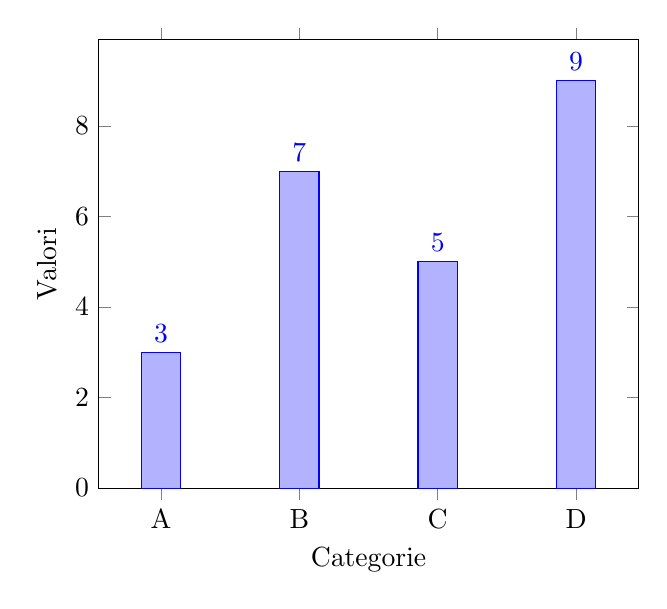
\begin{tikzpicture} 
        \begin{axis}[ 
            ybar, % Grafico a
            symbolic x coords={A, B, C, D}, % Etichette sull'asse x
            xtick=data, % Etichette dell'asse x corrispondono ai dati 
            ymin=0, % Valore
            ylabel={Valori}, % Etichetta dell'asse y 
            xlabel={Categorie}, 
            bar width=0.5cm, % Larghezza delle barre 
            nodes near coords,
            enlarge x limits=0.15 % Spazio aggiuntivo agli estremi
        ] 
        \addplot coordinates {(A,3) (B,7) (C,5) (D,9)}; 
        \end{axis}
    \end{tikzpicture} 
    \caption{Esempio di istogramma con dati fittizi.} 
\end{figure}


\newpage
\section{Tuttavia}

Notiamo che non ci sono enormi differenze in termini di tempi ma è presente un 
notevole aumento in termini della dimensione in particolare per quanto riguarda l'autenticazione.
E in contesto di questo tipo non è auspicabile

Cercando di trovare possibili soluzioni, ci siamo imbattuti su quello che è minimal IKE ovvero
una versione di IKE applicabile in scenari soggetti a constraint di risorse simili a quelli presenti nello spazio.

Riguardo a questo non esistono implementazioni, per questo motivo siamo passati a provare a dare un'implementazione di quest'ultimo
In modo tale che rappresenti un punto di inizio per questo scenario

Di questo trattiamo nel prossimo capitolo

%-----------------------------------
%	SECTION 3
%-----------------------------------

